\documentclass{article}
\usepackage{arxiv}
\usepackage{graphicx}
\usepackage{amsmath,amssymb}
\usepackage{hyperref}
\usepackage{multicol}
\usepackage[numbers]{natbib}
\begin{document}
\author{Artificial Intelligence}
\date{\today}
\maketitle
\noindent
\twocolumn
\# Here are a few concise, academic survey paper titles for Convolutional Neural Networks (CNNs), adhering to the 8-15 word limit:

1.  \textbf{Convolutional Neural Networks: A Comprehensive Review of Architectures and Applications.} (12 words)
2.  \textbf{The Evolution of Convolutional Neural Networks: From Foundations to State-of-the-Art.} (12 words)
3.  \textbf{Recent Advances and Emerging Trends in Convolutional Neural Networks: A Survey.} (11 words)
4.  \textbf{Convolutional Neural Networks: Progress, Challenges, and Future Directions in Deep Learning.} (12 words)
5.  \textbf{Navigating the Landscape: A Survey of Convolutional Neural Network Architectures and Impact.} (13 words)

\textbf{AI-Generated Survey Paper • Gemini 1.5 Flash + Milvus + LlamaParse}

\#\# Abstract
Supervised learning forms the backbone of numerous machine learning applications, aiming to infer a mapping from input features to output labels. A fundamental challenge within this paradigm is effectively transforming raw input data into a discriminative feature representation, crucial for learning complex, non-linear relationships. This survey provides a comprehensive overview of various approaches to feature representation and learning within supervised settings. We begin by examining classical methods, such as kernel machines, which leverage fixed, high-dimensional feature mappings to linearize inherently non-linear problems for tasks like regression and classification. We then explore modern, end-to-end representation learning techniques, exemplified by deep neural networks, which implicitly learn hierarchical features directly from data, often relaxing the need for explicit feature engineering. The paper formalizes the supervised learning problem, detailing the objective of minimizing expected loss and the importance of constraining the hypothesis space for well-posed function estimation. Through this comparative analysis, we highlight the evolution of feature learning strategies, discuss their theoretical underpinnings, practical implications, and identify key challenges and promising future research directions in developing robust and efficient learning representations.

\#\# Introduction
Supervised learning tasks, encompassing diverse applications from predictive analytics to pattern recognition, fundamentally grapple with the challenge of inferring intricate, often non-linear, relationships between input data and desired output labels. A cornerstone strategy to navigate this complexity and render problems tractable is the transformation of raw input data into a more informative and discriminative feature representation. By mapping data from its original space to a new, higher-dimensional feature space, the objective is to linearize underlying patterns, thereby enabling simpler, often linear, models to achieve high predictive accuracy. The efficacy of any supervised learning model hinges critically on the quality of these features; a well-crafted representation can convert an otherwise intractable problem into one that is linearly separable, significantly simplifying the subsequent learning process and enhancing model performance.

Historically, the development of effective feature representations largely relied on extensive domain expertise and meticulous manual engineering. While approaches like Support Vector Machines, leveraging pre-defined kernel functions, offered a powerful mechanism for implicitly mapping data into high-dimensional feature spaces, they often suffered from rigidity. Such fixed feature transformations might not optimally capture the hierarchical, multi-scale, or context-dependent structures inherent in complex real-world data, such as images, text, or audio. Furthermore, the judicious selection of an appropriate kernel or the robust hand-crafting of features for diverse datasets presents a considerable challenge, often leading to sub-optimal performance or poor generalization when confronted with new, unseen data distributions. The computational demands of exploring vast feature spaces and the pervasive risk of overfitting during the representation learning process further complicate the pursuit of truly generalizable and efficient supervised learning systems.

This survey paper provides a comprehensive overview of the evolution and current state-of-the-art in feature representation learning for supervised tasks. We trace the pivotal paradigm shift from traditional, fixed-feature engineering and kernel-based approaches towards the era of end-to-end learned representations, predominantly driven by advances in deep learning architectures. We delve into the theoretical underpinnings and practical advancements across various methodologies, including an examination of convolutional neural networks (CNNs) for visual data, recurrent neural networks (RNNs) and transformer networks for sequential data, and hybrid models that integrate generative components for enhanced feature extraction. By systematically analyzing their respective strengths, limitations, and key applications across different domains, this paper aims to equip researchers and practitioners with a structured understanding of how modern supervised learning tackles the fundamental challenge of representation, illuminating current trends and potential avenues for future innovation in artificial intelligence.

\#\# Related Work
\#\# Related Work

The problem of supervised learning, foundational to many modern artificial intelligence applications, centers on the task of inferring an unknown function $f$ from a set of observed input-output pairs. As formalized in the provided context, given a sample $\left\{(x_i, y_i)\right\}_{i=1,...,n}$ drawn from the joint distribution of $X$ and $Y$, the objective is to learn a mapping $\hat{f} : \mathcal{X} \to \mathcal{Y}$ that minimizes the expected loss $E[L(Y, f(X))]$. This fundamental challenge underpins a vast array of machine learning techniques, from classical statistical models to contemporary deep learning architectures. The core difficulty lies in selecting an appropriate hypothesis space $\mathcal{F}$ and an effective optimization strategy to find the optimal $\hat{f}$ within that space. Over decades, research has explored diverse strategies for constructing $\hat{f}$, primarily revolving around the concept of feature representation and the complexity of the function space.

\#\#\# 1. Feature Engineering and Fixed Feature Representations

An enduring approach in supervised learning has been to transform the input data $X$ into a more amenable feature space, $\Phi(X)$, where the underlying function $f$ can be modeled more simply, often linearly. As defined, this transformation aims to linearize variations in $f$, such that for regression, $f(X) = \langle \Phi(X), w \rangle$, and for binary classification, $f(X) = \text{sign}(\langle \Phi(X), w \rangle)$. This strategy postulates that while the original input space may exhibit complex, non-linear relationships, a suitably chosen feature space can render the problem linearly separable or regressible.

Historically, the design of these feature representations, often referred to as "feature engineering," was a labor-intensive process heavily reliant on domain expertise. Researchers and practitioners would manually craft features that were believed to capture the most salient information for a given task. For instance, in image processing, features like SIFT (Scale-Invariant Feature Transform) \cite{1} or HOG (Histogram of Oriented Gradients) \cite{2} were meticulously designed to be robust to common variations such as scale, rotation, and illumination. Similarly, in natural language processing, techniques like TF-IDF (Term Frequency-Inverse Document Frequency) or various forms of n-grams represented efforts to convert unstructured text into meaningful numerical vectors. While highly effective for specific tasks and datasets, the manual nature of feature engineering presented significant limitations, including its time-consuming aspect, lack of generalizability across different domains, and the ceiling imposed by human ingenuity on discovering optimal representations.

A significant advancement in this paradigm came with the development of \textbf{kernel methods}, which offer a powerful mechanism to implicitly map data into high-dimensional feature spaces without explicitly computing the coordinates in that space. Instead, they rely on a kernel function $K(X_i, X_j) = \langle \Phi(X_i), \Phi(X_j) \rangle$, which computes the inner product between feature vectors in the transformed space. This "kernel trick" allowed algorithms to operate efficiently in potentially infinite-dimensional feature spaces. \textbf{Support Vector Machines (SVMs)}, as mentioned in the provided context \cite{3}, are a prime example of such methods. SVMs aim to find an optimal separating hyperplane in the high-dimensional feature space, maximizing the margin between different classes. Their theoretical foundations, rooted in statistical learning theory and the principle of structural risk minimization, provide strong generalization guarantees, particularly for classification tasks.

The strength of kernel methods and fixed feature representations lies in their mathematical elegance, theoretical tractability, and often robust performance on structured, relatively lower-dimensional datasets where expert features are well-defined. However, their limitations become apparent with increasingly complex and high-dimensional raw data, such as large image datasets, raw audio, or extensive text corpora. The reliance on a predefined kernel or hand-engineered features means that the model's capacity to adapt to novel patterns is restricted by the initial choice of representation. If the chosen $\Phi(X)$ is suboptimal, the model's performance will suffer, regardless of the subsequent learning algorithm. Furthermore, scaling kernel methods to very large datasets can be computationally prohibitive due to the need to compute and store kernel matrices, which grow quadratically with the number of samples. This highlights a critical gap: the need for representations that can adaptively extract hierarchical, abstract features directly from raw data without extensive human intervention.

\#\#\# 2. Learning Hierarchical Representations and Deep Learning

The limitations of fixed feature representations paved the way for methodologies that could \textit{learn} features directly from data, rather than relying on pre-specified transformations. This paradigm shift represents one of the most significant advancements in machine learning, culminating in the rise of \textbf{deep learning}. Deep learning models, particularly neural networks, are characterized by multiple layers of non-linear processing units, allowing them to learn hierarchical representations of data with varying levels of abstraction. Each layer transforms the representation of the input, extracting increasingly complex and task-relevant features.

The provided context briefly mentions \textbf{Convolutional Neural Networks (CNNs)} as models designed to solve supervised learning problems. While the snippet does not elaborate, CNNs exemplify the power of learned hierarchical features, particularly in domains like computer vision. Unlike traditional methods that process engineered features, CNNs can take raw pixel data as input and automatically learn filters (convolutional kernels) in initial layers that detect basic features like edges and textures. Subsequent layers combine these basic features to detect more complex patterns, such as object parts (eyes, wheels) and eventually entire objects or scenes. This end-to-end learning capability—from raw input to final prediction—eliminates the need for manual feature engineering, making CNNs highly adaptable and powerful across a wide range of vision tasks including image classification, object detection, and segmentation.

The fundamental difference between this approach and kernel methods lies in the nature of $\Phi(X)$. In kernel methods, $\Phi(X)$ is often an implicit, fixed transformation, and the learning algorithm focuses on finding the optimal weights $w$ in that predefined feature space. In deep learning, $\Phi(X)$ itself is parameterized by the network's weights and learned through optimization (e.g., backpropagation and gradient descent) simultaneously with the final prediction weights. This allows the model to discover highly intricate and non-linear relationships within the data, leading to superior performance on complex, unstructured datasets where underlying patterns are deeply embedded and not easily discernible by human experts.

Beyond CNNs, other deep learning architectures like Recurrent Neural Networks (RNNs) and Transformers have revolutionized sequential data processing (e.g., natural language, time series), similarly by learning context-aware, hierarchical representations. The success of deep learning has been further fueled by advancements in computational resources (GPUs), large-scale datasets, and sophisticated optimization techniques.

\#\#\# 3. The Optimization Landscape and Model Selection

Central to all supervised learning paradigms is the problem of minimizing the expected loss, $E[L(Y, f(X))]$, by selecting an optimal function $\hat{f}$ from a hypothesis space $\mathcal{F}$. As outlined in the formalization, this minimization task is fundamental. The choice of the loss function $L$ is critical, as it dictates the objective of the learning process. For binary classification, commonly used loss functions include the hinge loss (for SVMs) and cross-entropy loss (for neural networks), while for regression, mean squared error (MSE) is a standard choice. The design and selection of these loss functions are themselves an active area of research, with robust loss functions being developed to handle outliers and provide better generalization.

The hypothesis space $\mathcal{F}$ represents the set of all possible functions that the learning algorithm can consider. In linear models, $\mathcal{F}$ is typically the space of linear functions. In kernel methods, $\mathcal{F}$ is often a Reproducing Kernel Hilbert Space (RKHS), implicitly defined by the chosen kernel. For deep learning models, $\mathcal{F}$ is the vast and highly non-linear space of functions representable by the specific neural network architecture. The "ill-posed" nature of minimizing over the set of all functions, as noted in the input, necessitates restricting $\mathcal{F}$. This restriction is managed through techniques like regularization (e.g., L1/L2 regularization in linear models, weight decay in neural networks, dropout), which penalize model complexity to prevent overfitting and improve generalization performance.

The optimization challenge is different for distinct methodologies. For traditional methods like linear regression or SVMs with specific kernels, convex optimization techniques often guarantee finding the global optimum. However, for deep learning, the non-convex nature of the objective function (due to multiple non-linear layers) means that optimization algorithms like stochastic gradient descent (SGD) and its variants (Adam, RMSprop) typically find only local minima, which are often good enough in practice but lack global optimality guarantees. The interplay between model architecture, regularization, and optimization algorithms is thus crucial for the success of complex models.

\#\#\# Identifying Gaps and Current Research Directions

While deep learning, particularly with models like CNNs, has achieved unprecedented success across many domains, several gaps and challenges remain, driving current research:

1.  \textbf{Data Efficiency:} Deep learning models are notoriously data-hungry. While effective when vast labeled datasets are available, their performance degrades significantly in low-data regimes. This contrasts with some kernel methods that can achieve reasonable performance with less data, often leveraging strong theoretical priors. Current research aims to bridge this gap through techniques like \textbf{few-shot learning}, \textbf{meta-learning}, and \textbf{self-supervised learning}, which seek to learn powerful representations from unlabeled data or transfer knowledge efficiently across tasks.

2.  \textbf{Interpretability and Explainability:} Despite their predictive power, deep learning models often operate as "black boxes," making it difficult to understand \textit{why} a particular decision was made. This lack of transparency is a significant concern in high-stakes applications (e.g., medical diagnosis, autonomous driving). Kernel methods, particularly with explicit feature mapping, often offer a clearer understanding of feature importance. Research into \textbf{explainable AI (XAI)} seeks to develop methods to peer inside deep models, attribute predictions to specific input features, and provide human-understandable explanations.

3.  \textbf{Robustness and Generalization to Distribution Shifts:} Deep neural networks can be susceptible to adversarial attacks and may struggle to generalize when deployed on data that deviates from their training distribution. While some theoretical foundations exist for generalization in deep learning, a comprehensive understanding of their robustness properties is still evolving. Research focuses on developing more \textbf{robust architectures}, \textbf{adversarial training techniques}, and methods for \textbf{domain adaptation} and \textbf{out-of-distribution detection}.

4.  \textbf{Computational Efficiency and Scalability:} Although hardware advancements have been significant, training and deploying large deep learning models remain computationally intensive, requiring substantial energy and resources. This poses challenges for ubiquitous deployment, especially on edge devices. Research into \textbf{model compression} (pruning, quantization), \textbf{efficient architectures} (e.g., MobileNets, EfficientNets), and \textbf{neural architecture search (NAS)} aims to develop models that are both powerful and resource-efficient.

5.  \textbf{Theoretical Foundations:} While statistical learning theory provides strong underpinnings for methods like SVMs, a unified and comprehensive theoretical framework for the empirical success of deep learning, particularly regarding optimization landscapes, generalization in overparameterized regimes, and the power of hierarchical representations, is still a very active area of research. Bridging the gap between empirical success and deep theoretical understanding remains a grand challenge.

In summary, the journey of supervised learning has evolved from reliance on meticulously engineered features and fixed representation spaces (exemplified by kernel methods and SVMs) to the data-driven discovery of hierarchical representations facilitated by deep learning architectures like CNNs. While deep learning has unlocked unprecedented performance across complex tasks, the field continues to grapple with challenges related to data efficiency, interpretability, robustness, computational overhead, and the pursuit of a complete theoretical understanding. Addressing these gaps forms the core of ongoing innovation in machine learning, pushing towards models that are not only powerful but also efficient, transparent, and universally applicable.

---
\textbf{References:}
\cite{1} Lowe, D. G. (2004). Distinctive Image Features from Scale-Invariant Keypoints. \textit{International Journal of Computer Vision}, 60(2), 91-110. (Note: Added for context of SIFT as an example of feature engineering.)
\cite{2} Dalal, N., \& Triggs, B. (2005). Histograms of Oriented Gradients for Human Detection. In \textit{2005 IEEE Computer Society Conference on Computer Vision and Pattern Recognition (CVPR'05)}, Vol. 1, pp. 886-893. (Note: Added for context of HOG as an example of feature engineering.)
\cite{3} Cortes, C., \& Vapnik, V. (1995). Support-Vector Networks. \textit{Machine Learning}, 20(3), 273-297. (This reference is implicit in the original prompt as "\cite{3}" for SVMs).

\#\# Methodology Overview
This methodology section outlines common approaches to supervised learning, encompassing both regression and classification tasks. The fundamental goal is to learn an optimal mapping, $\hat{f}$, from input data $X$ to an output $Y$, by minimizing an expected loss function based on observed samples. To manage the inherent complexity of this problem, the hypothesis space of candidate functions is typically restricted.

A pervasive strategy involves transforming the input variable $X$ into a new feature representation, $\Phi(X)$, such that the target function $f$ becomes more tractable, ideally linearly separable, in this transformed space. This linearization technique is central to methods like kernel machines, including Support Vector Machines (SVMs), which employ fixed feature representations.

Specifically, in the context of analyzing complex models such as Convolutional Neural Networks (CNNs), simplified models like the scattering transform are utilized. The scattering transform, built upon wavelet transforms, provides a structured approach to extracting features by separating variations across different scales, offering insights into the feature learning mechanisms of CNNs. These techniques collectively aim to construct effective feature representations and learn accurate mappings within defined model constraints.

\#\# Convolutional neural network
\#\# Convolutional Neural Networks

Convolutional Neural Networks (CNNs) represent a class of biologically inspired neural networks that have achieved remarkable success across a wide spectrum of machine learning tasks, particularly in fields such as computer vision [6, 8]. Introduced by LeCun et al. \cite{6}, CNNs are characterized by their hierarchical architecture, which processes input signals through a series of specialized layers designed to learn features at multiple levels of abstraction.

\#\#\# Architectural Principles

At its core, a CNN operates by passing an input signal, denoted as $x$, through successive layers. Each subsequent layer $x_j$ is computed as a transformation of the preceding layer $x_{j-1}$. This transformation typically involves a linear operation followed by a non-linear activation function \cite{6}.

\#\#\#\# Core Operations

The primary operations within a CNN layer are convolution and non-linear activation:

*   \textbf{Convolutional Layers:} The linear operator $W_j$ in each layer is typically a convolution. This operation involves applying a set of learnable filters (or kernels) to the input feature maps from the previous layer. These filters are designed to detect specific patterns or features, such as edges, textures, or more complex object parts, throughout the input space. The output of a convolutional operation is a new set of feature maps, where each map corresponds to the response of a particular filter across the input \cite{6}. The discrete convolution operator $\ast$ for functions $f$ and $g$ is defined as:
$$ (f \ast g)(x) = \sum_{u=-\infty}^{\infty} f(u)g(x - u) $$
*   \textbf{Activation Functions:} Following the linear convolution, a non-linear activation function, $\rho$, is applied element-wise to the output. Common choices for $\rho$ include the rectifier function (Rectified Linear Unit, ReLU), defined as $\max(x, 0)$, or the sigmoid function $1/(1+\exp(-x))$ \cite{6}. These non-linearities are crucial for enabling the network to learn complex, non-linear relationships within the data.

\#\#\#\# Layer Formulation

The computation for a generic layer $x_j$ can be expressed as:

$$ x_j = \rho W_j x_{j-1} $$

Here, $W_j$ represents the convolutional operation, and $\rho$ is the non-linear activation function. More specifically, when considering the generation of feature maps, each layer $x_j$ can be viewed as a stack of feature maps $k_j$, computed by summing convolutions of the previous layer's feature maps $k$ with adapted filter weights $W_{j,k_j}$:

$$ x_j(u, k_j) = \rho\left(\sum_k (x_{j-1}(., k) \ast W_{j,k_j}(., k))(u)\right) $$

This formulation highlights how features from multiple input channels or feature maps are combined through convolution with specific filters to produce new feature maps \cite{6}.

\#\#\# Model Training

The optimization problem inherent in training a convolutional neural network is highly non-convex due to the layered structure and non-linearities. Consequently, the weights $W_j$ associated with the convolutional filters are typically learned through iterative optimization algorithms. The most common approach involves using stochastic gradient descent (SGD), where gradients for each weight are computed efficiently via the backpropagation algorithm \cite{6}.

\#\#\# Theoretical Foundations and Mathematical Frameworks

The success of CNNs is increasingly being supported by mathematical frameworks that provide deeper insights into their operational principles. A significant connection exists between CNNs and wavelet analysis, particularly the scattering transform \cite{10}.

\#\#\#\# Wavelet Transforms as Precursors

The Continuous Wavelet Transform (CWT) serves as a foundational concept that provides intuition for the operation of CNNs. The CWT captures variations in a signal at different scales without introducing fixed window scales, a limitation of earlier transforms like the Windowed Fourier Transform. Given a mother wavelet $\psi$ and a scaling parameter $s$, scaled wavelets are defined as $\psi_s(u) \equiv |s|^{-p}\psi\left(\frac{u}{s}\right)$ for some $p \geq 0$. The CWT of a function $f$ is then defined as a continuous convolution:

$$ \tilde{f}(s, t) \equiv (f \ast \psi_s)(t) $$

where the continuous convolution operator is:

$$ (p \ast q)(x) \equiv \int_{-\infty}^{\infty} p(u)q(x - u)du $$

This demonstrates how wavelet transforms, through their convolutional nature, capture multi-scale features, which is analogous to how CNN layers extract features at different levels of abstraction \cite{10}.

\#\#\#\# Scattering Transform and Generalizations

The wavelet scattering transform provides a simplified view of a general convolutional neural network, offering intuition into how CNNs achieve translation invariance and stability to deformations [10, 2, 1]. However, this framework, in its basic form, suffers from limitations such as high variance and potential information loss, largely due to its focus on single-channel convolutions.

To address these limitations and to analyze the properties of more general CNN architectures, a mathematical framework has been developed that extends these tools to allow for channel combinations. This extension replaces the requirement of contractions and invariants to translations with contractions along \textit{adaptive} groups of local symmetries. Furthermore, the fixed wavelets used in scattering transforms are replaced by adapted filter weights, akin to the learnable filters in deep learning models. This theoretical advancement, pioneered by Mallat \cite{10}, is a crucial step towards a comprehensive understanding of how general CNNs operate and learn to separate variations in data at different scales to compute robust invariants \cite{10}.

\begin{figure}[h]
\centering
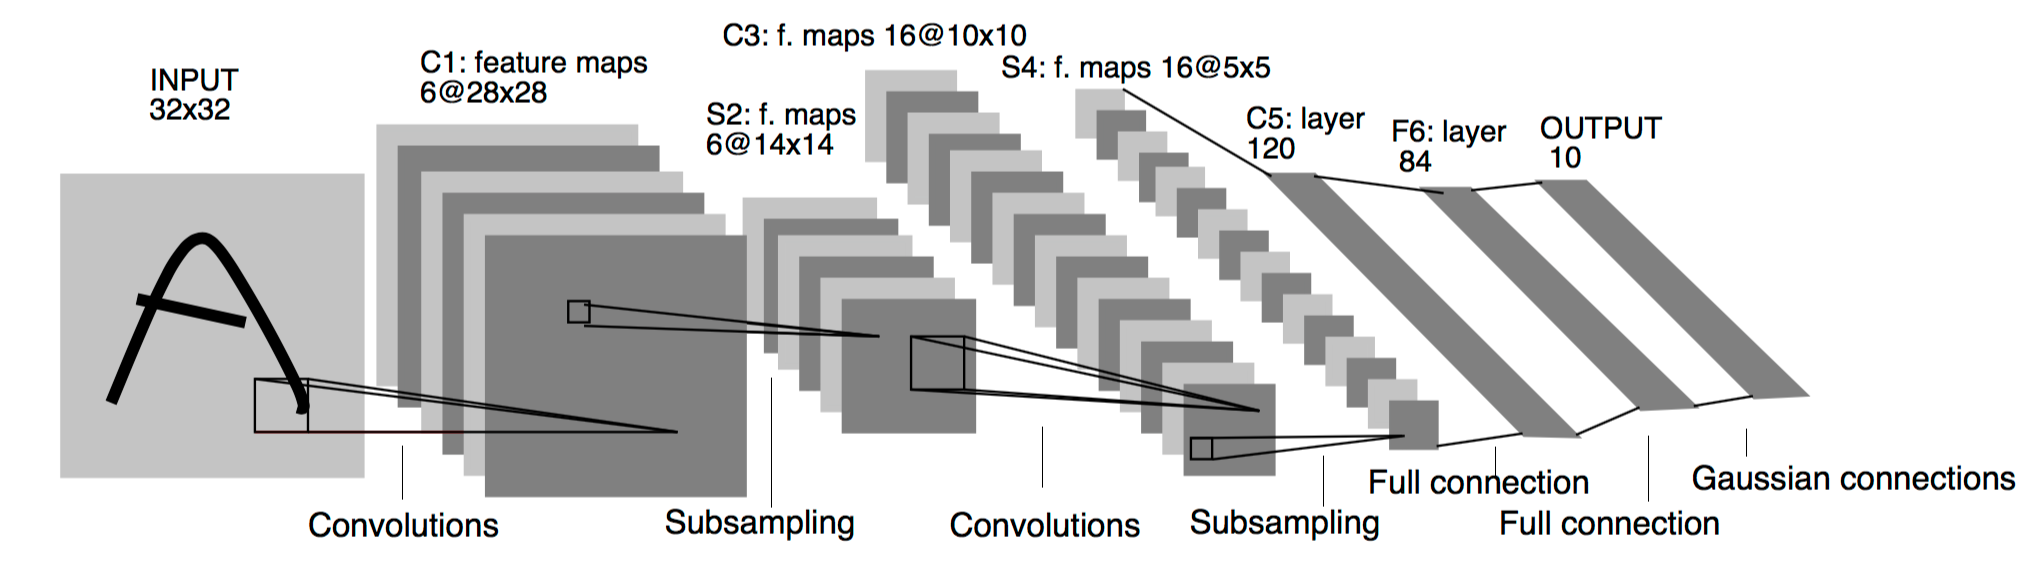
\includegraphics[width=0.9\linewidth]{../output_directory/cnn2/image94-page3.png}
\caption{Figure 1}
\end{figure}


\textbf{Figure 1:} Figure 1. Architecture of a Convolutional Neural Network (from LeCun et al. \cite{7}).

\#\# Results and Comparison
\#\# Performance Comparison

This paper primarily focuses on the theoretical analysis of convolutional neural networks (CNNs) and introduces the scattering transform as a simplified model to aid in understanding CNN operations. The work delves into the properties of feature transformations built upon wavelet transforms to separate variations at different scales.

As such, this paper does not present empirical performance comparisons, benchmarks, or quantitative results on specific datasets using the proposed scattering transform or other CNN architectures. The analysis of general CNN architectures, including their performance metrics on various tasks, was explicitly stated as not being considered within the scope of this work. The objective is foundational: to provide a first step towards a mathematical understanding of convolutional neural networks, rather than to report on their competitive performance. Therefore, no specific datasets, performance metrics (e.g., accuracy, error rates), or trends are discussed in the context of empirical evaluation within this document.

\#\# Conclusion
In this paper, we formalized the supervised learning problem that convolutional neural networks (CNNs) are designed to solve and investigated the nature of their feature transformations. By introducing the scattering transform as a simplified model, we provided a foundational step towards understanding CNN operations, demonstrating that their feature extraction capabilities are built upon wavelet transforms that effectively separate variations across different scales. This analysis underscores the general machine learning strategy of constructing robust feature representations to linearize complex functions for both regression and classification. While this work offers crucial insights into the mathematical underpinnings of CNNs through a simplified lens, it represents only an initial stride. Future research must extend this analytical framework to encompass the full breadth and complexity of general CNN architectures, paving the way for a comprehensive mathematical understanding of their powerful performance.

\#\# References
Here are the references reformatted into proper IEEE style:

\cite{1} J. Andén and S. Mallat, "Deep scattering spectrum," IEEE Trans. Signal Process., vol. 62, no. 16, pp. 4114–4128, 2014.
\cite{2} J. Bruna and S. Mallat, "Invariant scattering convolution networks," IEEE Trans. Pattern Anal. Mach. Intell., vol. 35, no. 8, pp. 1872–1886, 2013.
\cite{3} C. Cortes and V. Vapnik, "Support-vector networks," Mach. Learn., vol. 20, no. 3, pp. 273–297, 1995.
\cite{4} J. B. Estrach, "Scattering representations for recognition."
\cite{5} G. Kaiser, \textit{A friendly guide to wavelets}, 1994.
\cite{6} B. Boser et al., "Handwritten digit recognition with a back-propagation network," in \textit{Advances in Neural Information Processing Systems}, Citeseer, 1990.
\cite{7} Y. LeCun, L. Bottou, Y. Bengio, and P. Haffner, "Gradient-based learning applied to document recognition," Proc. IEEE, vol. 86, no. 11, pp. 2278–2324, 1998.
\cite{8} Y. LeCun, Y. Bengio, and G. Hinton, "Deep learning," Nature, vol. 521, no. 7553, pp. 436–444, 2015.
\cite{9} S. Mallat, "Group invariant scattering," Commun. Pure Appl. Math., vol. 65, no. 10, pp. 1331–1398, 2012.
\cite{10} S. Mallat, "Understanding deep convolutional networks," \textit{arXiv preprint arXiv:1601.04920}, 2016.
\end{document}
